%%%%%%%%%%%%%%%%%%%%%%%%%%%%%% Preamble
\documentclass{article}
\usepackage{amsmath,amssymb,amsthm,fullpage}
\usepackage[a4paper,bindingoffset=0in,left=1in,right=1in,top=1in,
bottom=1in,footskip=0in]{geometry}
\newtheorem*{prop}{Proposition}
\newenvironment{discussion}{\noindent Discussion.}{}
\setlength{\headheight}{12pt}
\setlength{\headsep}{10pt}
\usepackage{fancyhdr}
\usepackage{bbm}

% For images
\usepackage{graphicx}
\graphicspath{{images/}}

% For decision trees
\usepackage{tikz}
\usetikzlibrary{positioning}
\newdimen\nodeDist
\nodeDist=35mm

\pagestyle{fancy}
\fancyhf{}
\lhead{CS155 Homework 3}
\rhead{Matt Lim}
\begin{document}
%%%%%%%%%%%%%%%%%%%%%%%%%%%%%% Problem 1
\section*{Problem 1: Decision Tree Basic Questions}
\subsection*{Note: Using log base 2}
\subsection*{Note: Used entropy.py to calculate entropies}
\subsection*{1.}
\subsubsection*{(a)}
\textbf{Root}

For the root, we have that $S_1 = \{ No, Yes, Yes, Yes \}$ with $p_{S_1} = .75$,
which means we have an entropy of
\[ L(S) = 4 \cdot 0.811278124459 = 3.245112497836 \]

\noindent \textbf{Depth-1}

Splitting on Package type would give us \\
Bagged: $S_1 = \{ Yes, Yes \}$ with $p_{S_1} = 1$ \\
Canned: $S_2 = \{ No, Yes \}$ with $p_{S_2} = 0.5$ \\
This means we have an entropy of
\[ L(S) = L(S_1) + L(S_2) = 2 \cdot 0 + 2 \cdot 1.0 = 2.0 \]

Splitting on Unit price $> \$5$ would give us \\
Yes: $S_1 = \{ No, Yes \}$ with $p_{S_1} = 0.5$ \\
No: $S_2 = \{ Yes, Yes \} $ with $p_{S_2} = 1$ \\
This means we have an entropy of
\[ L(S) = L(S_1) + L(S_2) = 2 \cdot 1.0 + 2 \cdot 0 = 2.0 \]

Splitting on Contains $> 5$ grams of fat would give us \\
Yes: $S_1 = \{ No, Yes \}$ with $p_{S_1} = 0.5$ \\
No: $S_2 = \{ Yes, Yes \}$ with $p_{S_2} = 1$ \\
This means we have an entropy of
\[ L(S) = L(S_1) + L(S_2) = 2 \cdot 1.0 + 2 \cdot 0 = 2.0 \]

Since these all have the same entropy and we are using information gain as the splitting
criteria, we can pick any of the splits to use. We will pick the second (Unit price).
Note that we only need to split $S_1$ because $S_2$ is already completely pure.

\noindent \textbf{Depth-2}

Splitting on Package type would give us \\
Bagged: $S_1 = \{ Yes \} $ with $p_{S_1} = 1$ \\
Canned: $S_2 = \{ No \}$ with $p_{S_2} = 0$ \\
This means we have an entropy of
\[ L(S) = L(S_1) + L(S_2) = 1 \cdot 0 + 1 \cdot 0 = 0 \]

Splitting on Contains $> 5$ grams of fat would give us \\
Yes: $S_1 = \{ No \}$ with $p_{S_1} = 0$ \\
No: $S_2 = \{ Yes \}$ with $p_{S_2} = 1$ \\
This means we have an entropy of
\[ L(S) = L(S_1) + L(S_2) = 1 \cdot 0 + 1 \cdot 0 = 0 \]

\subsubsection*{(b)}
\noindent \textbf{Split-1}

We can see from above that our information gain is as follows:
\[ \text{Information Gain} = L(S_{root}) - (L(S_{1_{depth-1}}) + L(S_{2_{depth-1}})) =
    3.245112497836 - 2.0 = 1.2451124978360002 \]

\noindent \textbf{Split-2}

We can see from above that our information gain is as follows:
\[ \text{Information Gain} = L(S_{depth-1}) - (L(S_{1_{depth-2}}) + L(S_{2_{depth-2}})) =
    2.0 - 0 = 2.0 \]

\subsection*{(c)}
\begin{tikzpicture}[
    node/.style={%
      draw,
      rectangle,
    },
  ]

    \node [node] (A) {Unit Price $>$ 5};
    \path (A) ++(-135:\nodeDist) node [node] (B) {Contains $>$ 5 grams of fat};
    \path (A) ++(-45:\nodeDist) node [node] (C) {1};
    \path (B) ++(-135:\nodeDist) node [node] (D) {0};
    \path (B) ++(-45:\nodeDist) node [node] (E) {1};

    \draw (A) -- (B) node [left,pos=0.25] {yes}(A);
    \draw (A) -- (C) node [right,pos=0.25] {no}(A);
    \draw (B) -- (D) node [left,pos=0.25] {yes}(A);
    \draw (B) -- (E) node [right,pos=0.25] {no}(A);
\end{tikzpicture}

\vspace{5mm}

\noindent Step 1: $L(S) = 3.245112497836$ \\
Step 2: $L(S) = 2.0$  \\
Step 3: $L(S) = 0.0$ \\

\subsection*{(d)}
\subsubsection*{Impurities Using Gini Index}
\textbf{Root}

For the root, we have that $S_1 = \{ No, Yes, Yes, Yes \}$ with $p_{S_1} = .75$,
which means we have an impurity of
\[ L(S) = 4 \cdot 0.375 = 1.5 \]

\noindent \textbf{Depth-1}

Splitting on Package type would give us \\
Bagged: $S_1 = \{ Yes, Yes \}$ with $p_{S_1} = 1$ \\
Canned: $S_2 = \{ No, Yes \}$ with $p_{S_2} = 0.5$ \\
This means we have an impurity of
\[ L(S) = L(S_1) + L(S_2) = 2 \cdot 0 + 2 \cdot 0.5 = 1.0 \]

Splitting on Unit price $> \$5$ would give us \\
Yes: $S_1 = \{ No, Yes \}$ with $p_{S_1} = 0.5$ \\
No: $S_2 = \{ Yes, Yes \} $ with $p_{S_2} = 1$ \\
This means we have an impurity of
\[ L(S) = L(S_1) + L(S_2) = 2 \cdot 0.5 + 2 \cdot 0 = 1.0 \]

Splitting on Contains $> 5$ grams of fat would give us \\
Yes: $S_1 = \{ No, Yes \}$ with $p_{S_1} = 0.5$ \\
No: $S_2 = \{ Yes, Yes \}$ with $p_{S_2} = 1$ \\
This means we have an impurity of
\[ L(S) = L(S_1) + L(S_2) = 2 \cdot 0.5 + 2 \cdot 0 = 1.0 \]

Since these all have the same impurity and we are using information gain as the splitting
criteria, we can pick any of the splits to use. We will pick the second (Unit price).
Note that we only need to split $S_1$ because $S_2$ is already completely pure.

\noindent \textbf{Depth-2}

Splitting on Package type would give us \\
Bagged: $S_1 = \{ Yes \} $ with $p_{S_1} = 1$ \\
Canned: $S_2 = \{ No \}$ with $p_{S_2} = 0$ \\
This means we have an impurity of
\[ L(S) = L(S_1) + L(S_2) = 1 \cdot 0 + 1 \cdot 0 = 0 \]

Splitting on Contains $> 5$ grams of fat would give us \\
Yes: $S_1 = \{ No \}$ with $p_{S_1} = 0$ \\
No: $S_2 = \{ Yes \}$ with $p_{S_2} = 1$ \\
This means we have an impurity of
\[ L(S) = L(S_1) + L(S_2) = 1 \cdot 0 + 1 \cdot 0 = 0 \]

\subsubsection*{Information Gain}
\noindent \textbf{Split-1}

We can see from above that our information gain is as follows:
\[ \text{Information Gain} = L(S_{root}) - (L(S_{1_{depth-1}}) + L(S_{2_{depth-1}})) =
    1.5 - 1.0 = 0.5 \]

\noindent \textbf{Split-2}

We can see from above that our information gain is as follows:
\[ \text{Information Gain} = L(S_{depth-1}) - (L(S_{1_{depth-2}}) + L(S_{2_{depth-2}})) =
    1.0 - 0.0 = 1.0 \]

\subsubsection*{Draw the Tree}

\begin{tikzpicture}[
    node/.style={%
      draw,
      rectangle,
    },
  ]

    \node [node] (A) {Unit Price $>$ 5};
    \path (A) ++(-135:\nodeDist) node [node] (B) {Contains $>$ 5 grams of fat};
    \path (A) ++(-45:\nodeDist) node [node] (C) {1};
    \path (B) ++(-135:\nodeDist) node [node] (D) {0};
    \path (B) ++(-45:\nodeDist) node [node] (E) {1};

    \draw (A) -- (B) node [left,pos=0.25] {yes}(A);
    \draw (A) -- (C) node [right,pos=0.25] {no}(A);
    \draw (B) -- (D) node [left,pos=0.25] {yes}(A);
    \draw (B) -- (E) node [right,pos=0.25] {no}(A);
\end{tikzpicture}

\vspace{5mm}

\noindent Step 1: $L(S) = 1.5$ \\
Step 2: $L(S) = 1.0$ \\
Step 3: $L(S) = 0.0$ \\

\newpage
\subsection*{2.}
Compared to a linear classifier, the decision tree is not always preferred for
classification problems. One example is the following.

\begin{figure}[h]
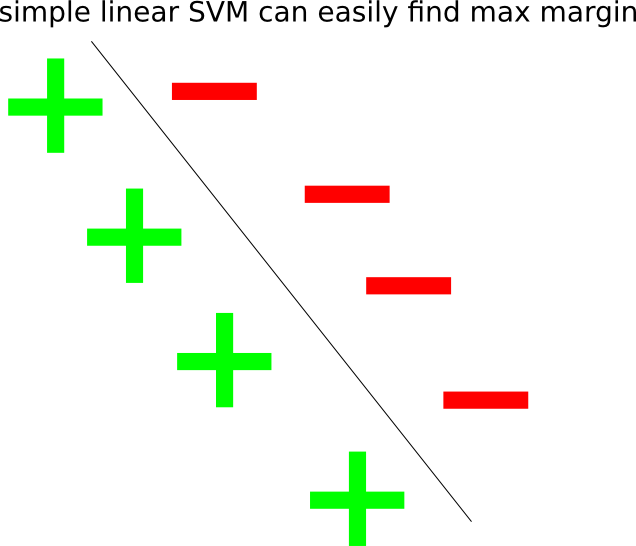
\includegraphics[width=8cm]{lin}
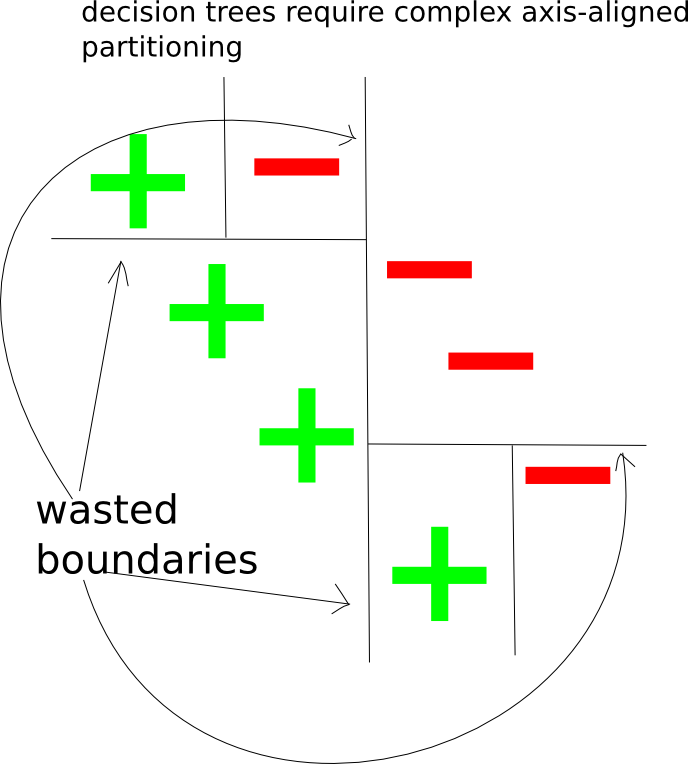
\includegraphics[width=8cm]{tree}
\end{figure}

\subsection*{3.}
\subsubsection*{(a)}
\textbf{Impurities Using Gini Index}

\noindent \textbf{Root}

For the root, we have that $p_{S_1} = 0.5$, which means we have an impurity of
\[ L(S) = 4 \cdot 0.5 = 2.0 \]

\noindent \textbf{Depth-1}

Splitting on $X_1$ would give us \\
$X_1 = 0$: $S_1 = \{ Neg, Pos \}$ with $p_{S_1} = 0.5$ \\
$X_1 = 1$: $S_2 = \{ Pos, Neg \}$ with $p_{S_2} = 0.5$ \\
This means we have an impurity of
\[ L(S) = L(S_1) + L(S_2) = 2 \cdot 0.5 + 2 \cdot 0.5 = 2.0 \]

Splitting on $X_2$ would give us \\
$X_2 = 0$: $S_1 = \{ Neg, Pos \}$ with $p_{S_1} = 0.5$ \\
$X_2 = 1$: $S_2 = \{ Pos, Neg \}$ with $p_{S_2} = 0.5$ \\
This means we have an impurity of
\[ L(S) = L(S_1) + L(S_2) = 2 \cdot 0.5 + 2 \cdot 0.5 = 2.0 \]

Since no split of the root results in any reduction in impurity, given our stopping
condition we do not split the root at all, and end up with a tree that is just a root node.
The resulting tree looks as follows, and has a classification error of $0.5$.

\vspace{5mm}
\begin{tikzpicture}[
    node/.style={%
      draw,
      rectangle,
    },
  ]

    \node [node] (A) {1 (root)};
\end{tikzpicture}

\subsubsection*{(b)}
\textbf{Classification Error as Impurity}

\noindent \textbf{Root}

For the root, we have an impurity of
\[ L(S) = 4 \cdot 0.5 = 2.0 \]
because the classification error is $0.5$.

\noindent \textbf{Depth-1}

Splitting on $X_1$ would give us \\
$X_1 = 0$: $S_1 = \{ Neg, Pos \}$, which means $E_{S_1} = 0.5$ \\
$X_1 = 1$: $S_2 = \{ Pos, Neg \}$, which means $E_{S_2} = 0.5$ \\
This means we have an impurity of
\[ L(S) = L(S_1) + L(S_2) = 2 \cdot 0.5 + 2 \cdot 0.5 = 2.0 \]
because the classification errors are $0.5$.

Splitting on $X_2$ would give us \\
$X_2 = 0$: $S_1 = \{ Neg, Pos \}$, which means $E_{S_1} = 0.5$ \\
$X_2 = 1$: $S_2 = \{ Pos, Neg \}$, which means $E_{S_2} = 0.5$ \\
This means we have an impurity of
\[ L(S) = L(S_1) + L(S_2) = 2 \cdot 0.5 + 2 \cdot 0.5 = 2.0 \]
because the classification errors are $0.5$.

Since no split of the root results in any reduction in the impurity, given our stopping
condition we do not split the root at all, and end up with a tree that is just a root node.
The resulting tree looks as follows, and has a classification error of $0.5$.

\vspace{5mm}
\begin{tikzpicture}[
    node/.style={%
      draw,
      rectangle,
    },
  ]

    \node [node] (A) {1 (root)};
\end{tikzpicture}

\subsubsection*{(c)}
In order to achieve zero classification training error, we need $99$ unique
thresholds (internal nodes) in the worst case.

One way to see this is to
see that in the worst case, the decision tree must have $100$ leaf nodes in order
to achieve zero classification training error. That is, in the worst case, we must split
each training point into its own leaf to achieve zero classification training error.
And by definition, a binary tree with $l$ leaf nodes has $n = 2l - 1$ nodes,
which means it has $l - 1 = 99$ internal nodes.

Another way to see this is that
adding one additional training point requires us to add only one additional
internal node. For example, say we have two training points. We can classify
these two with just one internal node and two leaf nodes. Then consider what happens
when we add another training point. This new training point will fall into
one of the existing leaf nodes (one of the existing splits). So all we need to do
in order to maintain zero classification training error is split that leaf node
into two new leaf nodes (the new training point will fall into one, the old will
fall into the other), which gives us one more internal node. This logic continues,
and we can see that for $100$ training points, we need $99$ internal nodes (since
we start with one internal node for two training points and add one internal node
for every additional training point).

\subsection*{4.}
The worst-case complexity of the number of possible splits we must consider is
\[ O(DN) \]
This is because given $N$ data points, there are $N-1$ possible positions at which
we can split them, and at each position, we can split using one of $D$ features/attributes (because
all of them are continuous).

\newpage
\section*{Problem 2: Implementation of Decision Tree}
\subsection*{Note: Used decision\_tree.py for this section}
\subsection*{1.}
\begin{figure}[h]
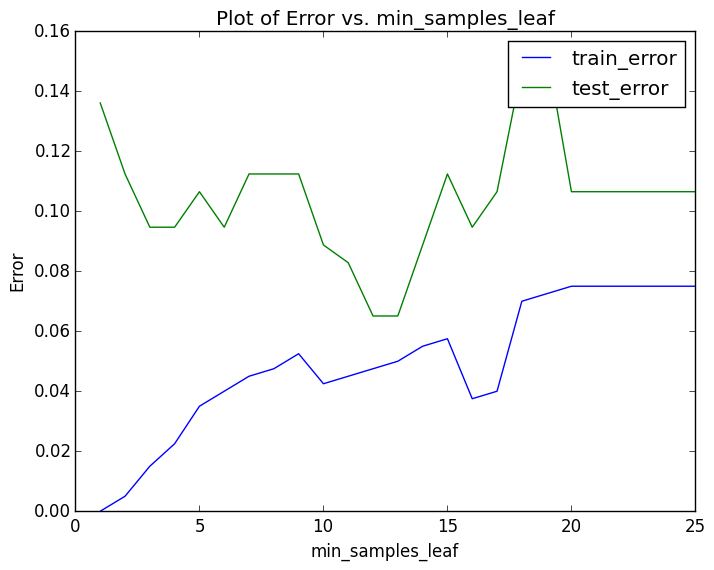
\includegraphics[width=8cm]{min_samples_leaves}
\end{figure}

\subsection*{2.}
\begin{figure}[h]
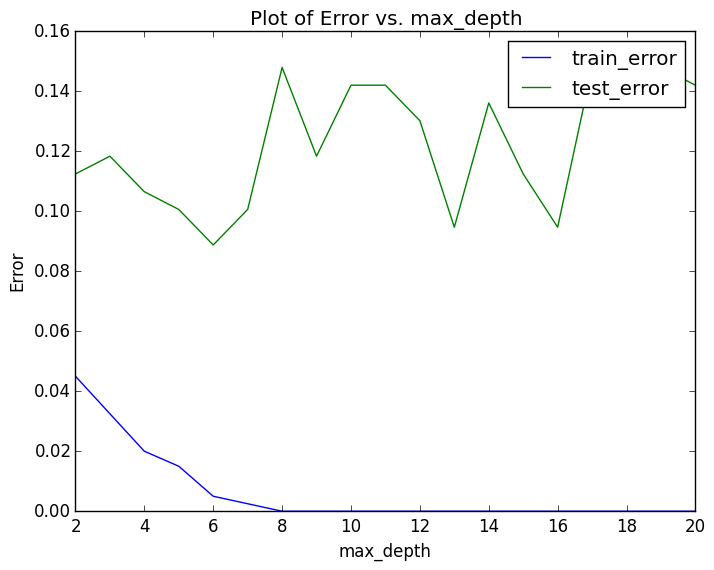
\includegraphics[width=8cm]{max_depths}
\end{figure}

\subsection*{3.}
Note that the graphs are not perfect and fluctuate quite a bit. This was most likely
caused by the relatively small sizes of our training/test data sets.

\subsubsection*{First Plot}
For the first plot, early stopping can be seen as we move right along the x-axis,
because a higher min\_samples\_leaf value means that the decision trees we end up with
have leaves with more points which in turn means the algorithm needed to use less splits
and thus stopped earlier.

We can see that when there is no early stopping (i.e. when min\_samples\_leaf = 1)
overfitting occurs, because training error goes down and test error goes up.
When there is early stopping (min\_samples\_leaf around 10-15), we can see that
training error rises but test error falls. Thus we can conclude that early stopping
helps prevent overfitting and improves generalization. However, when we stop too
early, we can see that both training error and test error rise, and that we
begin to underfit. So we need to make sure not to stop too early.

\subsubsection*{Second Plot}
For the first plot, early stopping can be seen as we move left along the x-axis,
because a lower max\_depth value means that the decision trees we end up with
are limited to less levels, which in turn means the algorithm needed to use less
splits and thus stopped earlier.

We can see that when there is no early stopping (i.e. when max\_depth $>$ 8)
overfitting occurs, because training error goes down and test error goes up.
When there is early stopping (max\_depth around 6-8), we can see that training error
rises but test error falls. Thus we can conclude that early stopping helps prevent overfitting and
improves generalization. However, when we stop too early, we can see that
both training error and test error rise, and that we begin to underfit. So we need
to make sure not to stop too early.

\newpage
\section*{Problem 3: The AdaBoost Algorithm}
\subsection*{(a)}
We want to show that
\[ E = \frac{1}{m} \sum_{i = 1}^m \exp(-y_i f(x_i)) \geq \frac{1}{m} \sum_{i = 1}^m
    \mathbbm{1} (H(x_i) \neq y_i) \]

To show this, it suffices to show that for each pair $x_i, y_i$,

\[ \exp(-y_i f(x_i)) \geq \mathbbm{1} (H(x_i) \neq y_i) \]

To show this, we just need to consider two cases. The first case is
if $y_i$ and $f(x_i)$ disagree in sign. In this case,
\[ \mathbbm{1} (H(x_i) \neq y_i) = 1 \]
\[ \exp(-y_i f(x_i)) = \exp(p) \]
where $p$ is a nonnegative number. And we know that
\[ \exp(x) \geq 1, x \geq 0 \]
So overall, we have that
\[ \exp(-y_i f(x_i)) \geq \mathbbm{1} (H(x_i) \neq y_i) \]

The next case is if $y_i$ and $f(x_i)$ agree in sign. In this case,
\[ \mathbbm{1} (H(x_i) \neq y_i) = 0 \]
\[ \exp(-y_i f(x_i)) = \exp(n) \]
where $n$ is a negative number. And we know that
\[ \exp(x) \geq 0, x \in \mathbb{R} \]
So overall, we have that
\[ \exp(-y_i f(x_i)) \geq \mathbbm{1} (H(x_i) \neq y_i) \]

Then we have that in both/all cases,
\[ \exp(-y_i f(x_i)) \geq \mathbbm{1} (H(x_i) \neq y_i) \]
Thus we can conclude that
\[ E = \frac{1}{m} \sum_{i = 1}^m \exp(-y_i f(x_i)) \geq \frac{1}{m} \sum_{i = 1}^m
    \mathbbm{1} (H(x_i) \neq y_i) \]

\subsection*{(b)}
We have from lecture that
\[ D_{t+1}(i) = \frac{D_t(i) \exp(-\alpha_t y_i h_t(x_i))}{Z_t} \]

So we can write any $D_t(i)$ as follows:

\[ D_t(i) = \Big( \prod_{j = 1}^{t - 1} \frac{\exp(-\alpha_j y_i h_j(x_i))}{Z_j} \Big)
    \cdot D_1(i) \]

Then we can write $Z_T$ as follows:

\[ Z_T = \sum_{i = 1}^m \Big( \prod_{j = 1}^{T - 1} \frac{\exp(-\alpha_j y_i h_j(x_i))}{Z_j} \Big)
    \cdot D_1(i) \cdot \exp(-\alpha_T y_i h_T(x_i)) \]

\[ Z_T = \sum_{i = 1}^m \Big( \prod_{j = 1}^{T - 1} \frac{1}{Z_j} \Big) \cdot
    \Big( \prod_{j = 1}^{T - 1} \exp(-\alpha_j y_i h_j(x_i)) \Big)
    \cdot D_1(i) \cdot \exp(-\alpha_T y_i h_T(x_i)) \]

\[ Z_T = \sum_{i = 1}^m \Big( \prod_{j = 1}^{T - 1} \frac{1}{Z_j} \Big) \cdot
    \Big( \prod_{j = 1}^{T} \exp(-\alpha_j y_i h_j(x_i)) \Big)
    \cdot D_1(i) \]

\[ Z_T = \sum_{i = 1}^m \Big( \prod_{j = 1}^{T - 1} \frac{1}{Z_j} \Big) \cdot
    \exp(-y_i \sum_{j = 1}^T \alpha_j h_j(x_i))
    \cdot D_1(i) \]

\[ Z_T = \sum_{i = 1}^m \Big( \prod_{j = 1}^{T - 1} \frac{1}{Z_j} \Big) \cdot
    \exp(-y_i f(x_i))
    \cdot D_1(i) \]

\[ \Big( \prod_{j = 1}^{T - 1} Z_j \Big) \cdot Z_T = \sum_{i = 1}^m
    \exp(-y_i f(x_i))
    \cdot D_1(i) \]

\[ \prod_{j = 1}^{T} Z_j = \sum_{i = 1}^m \exp(-y_i f(x_i)) \cdot D_1(i) \]

Finally, we can use the fact that we initialize $D_1(x) = \frac{1}{m}$ to
get the desired result.

\[ \prod_{j = 1}^{T} Z_j = \frac{1}{m} \sum_{i = 1}^m \exp(-y_i f(x_i)) \]

\subsection*{(c)}
Let $\epsilon_t$, the training set error of a weak classifier $h_t$ for a weighted
dataset, be given as follows:

\[ \epsilon_t = \sum_{i = 1}^m D_t(i) \mathbbm{1} (h_t(x_i) \neq y_i) \]

We will consider a special class of weak classifiers $h_t(x)$ that return exactly
$+1$ if $h_t$ classifies example $x$ as positive, and $-1$ if $h_t$ if classifies
$x$ as negative. We will show that for this class of classifiers the normalizer
$Z_t$ can be written as

\[ Z_t = (1 - \epsilon_t) \exp(-\alpha_t) + \epsilon_t \exp(\alpha_t) \]

We can see this is true by considering our only two cases. \\
First, we will consider when $h_t(x_i) \neq y_i \implies h_t(x_i) y_i = -1$.
In this case, we have that (since we always normalize our weightings such that
they sum to 1)
\[ \epsilon_t = \sum_{i = 1}^m D_t(i) = 1 \]
which means that, under our new definition,
\[ Z_t = \exp(\alpha_t) \]
We can see that under our old definition,
\[ Z_t = \sum_{i = 1}^m D_t(i) \exp(-\alpha_t y_i h_t(x_i)) \]
\[ Z_t = \sum_{i = 1}^m D_t(i) \exp(\alpha_t) \]
\[ Z_t = \exp(\alpha_t) \]
So in this case, the normalizer $Z_t$ can be written as desired.

Next, we will consider when $h_t(x_i) = y_i \implies h_t(x_i) y_i = 1$.
In this case, we have that
\[ \epsilon_t = 0 \]
which means that, under our new definition,
\[ Z_t = \exp(-\alpha_t) \]
We can see that under our old definition,
\[ Z_t = \sum_{i = 1}^m D_t(i) \exp(-\alpha_t y_i h_t(x_i)) \]
\[ Z_t = \sum_{i = 1}^m D_t(i) \exp(-\alpha_t) \]
Since we always normalize our weightings such that they sum to 1, this turns into
\[ Z_t = \exp(-\alpha_t) \]
So in this case, the normalizer $Z_t$ can be written as desired.

So in both/all cases, the normalizer can be written as desired. Now we will
minimize $Z_t$ with respect to $\alpha_t$.

\[ \frac{\delta Z_t}{\delta \alpha_t} = (1 - \epsilon_t)(-\alpha_t)\exp(-\alpha_t)
    + \epsilon_t \alpha_t \exp(\alpha_t) = 0 \]

\[ \epsilon_t \alpha_t \exp(\alpha_t) = \alpha_t (1 - \epsilon_t) \exp(-\alpha_t) \]

\[ \exp(2 \alpha_t) = \frac{1 - \epsilon_t}{\epsilon_t} \]

\[ \alpha_t = \frac{1}{2} \ln \Big(\frac{1 - \epsilon_t}{\epsilon_t} \Big) \]

\[ \implies \alpha^*_t = \frac{1}{2} \ln \Big(\frac{1 - \epsilon_t}{\epsilon_t} \Big) \]

Thus, we can see that choosing $\alpha_t$ to greedily minimize $Z_t$ leads to
the choices in AdaBoost. We also want to choose $h_t$ to greedily minimize
$Z_t$. Since the only variable in our expression for $Z_t$ that involves
$h_t$ is $\epsilon_t$, this means we just want to choose the model $h_t$ such
that $\epsilon_t$ minimizes $Z_t$.

\end{document}
